\documentclass[conference]{IEEEtran}
\usepackage[T1]{fontenc}
\usepackage{amsmath,amssymb}
\usepackage{graphicx,booktabs,array,balance}
\usepackage[hidelinks]{hyperref}
\usepackage{url}
\graphicspath{{figures/}}
\begin{document}
\title{Cross-City Transfer Learning for AQI Forecasting in Data-Scarce Indian Regions}
\author{\IEEEauthorblockN{Arjun Srikanth, Ankit Umadi, Jayanth K}
\IEEEauthorblockA{PES University, Bengaluru, India\\Team Toxic (Team 23)}}
\maketitle
\begin{abstract}
We forecast daily air quality index (AQI) in six held-out Indian cities using official Central Pollution Control Board records. Models use seven observed AQI values, three target fitting budgets and one- to three-day horizons. Model fitting ends in 2023, with evaluation in 2024 and 2025. On the 2025 test, compact pooled Transformer mean absolute error (MAE) is 22.24, 27.15 and 29.51 AQI points at one, two and three days, versus 23.12, 30.36 and 34.30 for persistence. Fine-tuning beats matching local training in 88 of 99 MAE comparisons. The full joint MAE/RMSE criterion against local training and persistence holds in 0 of 99 comparisons. Full MAML, first-order MAML and Reptile trail ordinary transfer in all 27 primary macro MAE comparisons. Post-hoc controls show that a tenfold smaller learning rate reduces the 2025 fine-tuning penalty across five architectures. On matched donor tasks, replacing the after-update MAML objective with immediate forecast loss accounts for 1.33 points of the original 1.59-point starting gap.
\end{abstract}
\begin{IEEEkeywords}
AQI forecasting, transfer learning, meta-learning, data scarcity, CPCB, chronological evaluation
\end{IEEEkeywords}

\section{Introduction}
An AQI forecasting model for a station with few fitting observations can use data from other locations in several ways. It can apply a pooled model directly, adapt pooled weights using the available target labels, or learn an initialization specifically for rapid adaptation. These choices answer different questions. A lower error than training a neural network from scratch may reflect the difficulty of fitting that network to a small sample. It does not establish that adaptation improves the original pooled model, or that either model improves a simple forecast.

This project studies those distinctions for daily overall AQI from the Central Pollution Control Board (CPCB). India's national AQI combines pollutant information into an index intended for public communication~\cite{cpcb_report}. We forecast the station index supplied by the official repository~\cite{cpcb_data}; we do not substitute a pollutant concentration, reconstruct AQI from unaligned covariates, or interpret one monitor as a citywide exposure estimate. The accepted project question concerns cross-city transfer under limited target data. We operationalize scarcity as a restriction on target labels used for fitting, while giving every method legal recent observed context at prediction time.

We ask three primary questions. First, does donor pretraining improve on local training and on persistence or a seven-day mean? Second, does target fine-tuning add value beyond applying the pooled model directly? Third, does meta-learning improve on ordinary transfer with a common backbone and adaptation optimizer? Post-hoc controls change the target learning rate across five architectures and isolate the MAML training objective on the original donor task stream.

We retain the source files, target fitting-label sets, predictions, model settings and independent metric checks. Pooled models improve on persistence most clearly at longer horizons. The matched experiments distinguish that gain from the effect of adapting to a small target sample.

\section{Related Work}
Cross-city transfer for data-scarce urban prediction predates this study. RegionTrans matches regions across cities and transfers spatiotemporal representations~\cite{regiontrans}. Its demonstration uses crowd flow; its reported improvement is not evidence about Indian AQI. Air-quality transfer has also been studied directly. Poelzl et al. investigate transfer for PM$_{10}$ prediction with limited target data~\cite{poelzl}. This establishes relevant prior art while differing from our overall-AQI target and Indian station cohort. Our study does not claim that cross-city transfer, limited-label evaluation or season-sensitive target histories are new ideas.

We compare recurrent, convolutional, attention and feedforward model families. Gated recurrent units~\cite{cho} and long short-term memory networks~\cite{lstm} encode sequential dependencies; temporal convolutional networks provide another sequence-modeling approach~\cite{tcn}; Transformer self-attention offers a nonrecurrent alternative~\cite{transformer}. These references motivate standard model families rather than certify that a particular architecture should win on seven daily inputs. A compact model is therefore retained when increasing capacity and optimization effort.

Model-agnostic meta-learning (MAML) trains parameters to perform well after a small number of task-specific gradient updates~\cite{maml}. First-order MAML omits second-order terms. Reptile instead moves an initialization toward task-adapted parameters~\cite{reptile}. These methods assume that the training tasks support useful adaptation on new tasks. Here, a city defines a task, and the small number of independent donor cities is a substantial limitation. We assess meta-learning against ordinary pretraining with a common differentiable GRU and native stochastic gradient descent (SGD) adaptation, rather than infer a meta-learning benefit from unmatched networks.

\section{Data and Evaluation Protocol}
\subsection{Source archive and quality checks}
The retained versioned release contains 3,820 daily AQI workbooks spanning 2017--2025 and 769,129 decoded station-date observations. Of these observations, 758,536 match station identities in the captured official metadata and 10,593 belong to separately retained unmatched IDs. The archive includes 1,059 empty workbooks. Four values above 500 occur in 2017; they remain visible in the source-quality record. Modeling starts in 2020. The extraction checks report no duplicate station-date readings or parse failures. Original workbooks are retained with checksums, and summary rows in spreadsheet layouts are excluded from daily observations.

The acquisition and modeling scopes must be distinguished. The release covers records obtained through the current CPCB station roster and indexed public exports. It is not a census of all historical Indian monitors or proof of uninterrupted operation. Empty files, unlisted station-years and missing daily values do not establish why data are unavailable. The forecasting experiment uses a selected subset, not all observations in the archive.

\subsection{Cohort construction and geographic separation}
Requiring at least 80\% observed daily values in every year from 2020 through 2025 leaves 60 stations representing 30 city codes. One representative per city is selected by the number of observed days in 2020--2023, with numeric station ID breaking ties. Six cities, in different states, form the target cohort: Amaravati, Guwahati, Ahmedabad, Pithampur, Ludhiana and Udaipur. They were chosen before inspecting the final experiment's target forecasts. This is a convenience and availability cohort, not random sampling of Indian cities.

Every station in a target city is excluded from donor fitting and selection. We additionally remove non-target representative stations within 25 km of any known station in a target city. This excludes Vatva near Ahmedabad and leaves 23 donor cities. The nearest retained donor is approximately 42.6 km from a target station. The buffer uses current coordinates; it does not prove historical station separation. Chandigarh, Dewas, Jalandhar and Ajmer are held-out development cities during preliminary fitting. They may join the final donor refit after settings are selected. Target-city data never select a setting.

Coverage-based selection uses availability through 2025 and thus favors consistently reporting monitors. Although test errors do not determine eligibility, this restriction conditions the population being evaluated. Furthermore, complete seven-day contexts reduce evaluation availability even at stations passing the annual threshold. Table~\ref{tab:cohort} shows the resulting target-date counts. Each listed date supplies all three horizons on common eligible labels.

\begin{table}[t]
\caption{Target stations and common eligible evaluation dates}
\label{tab:cohort}
\centering\small
\begin{tabular}{lrrr}\toprule
City & Station ID & 2024 dates & 2025 dates\\\midrule
Amaravati & 1406 & 240 & 266\\
Guwahati & 5073 & 177 & 135\\
Ahmedabad & 308 & 163 & 133\\
Pithampur & 1402 & 353 & 295\\
Ludhiana & 253 & 320 & 304\\
Udaipur & 1397 & 343 & 293\\\midrule
Total & & 1,596 & 1,426\\\bottomrule
\end{tabular}
\end{table}

\subsection{Forecast definition and scarcity budgets}
Let $y_{c,t}$ denote observed AQI at the representative monitor in city $c$ on issue day $t$. Each forecast uses seven consecutive observed AQIs,
\begin{equation}
\mathbf{x}_{c,t}=(y_{c,t-6},\ldots,y_{c,t}),
\end{equation}
plus issue-day annual and weekly sine/cosine phases and the horizon $h\in\{1,2,3\}$. Calendar phases use the issue day, not future observed information. AQI inputs are divided by 500, the horizon by three, and the residual target $(y_{c,t+h}-y_{c,t})$ by 100. These fixed scales require no estimated test statistics. Networks produce a direct horizon-conditioned residual,
\begin{equation}
\widehat y_{c,t+h}=y_{c,t}+100f_\theta(\mathbf{x}_{c,t}/500,\mathbf{k}_{t},h/3).
\end{equation}
Outputs are continuous and uncapped. We use no future measurements, weather or neighboring-station inputs. Missing inputs or truth make a window ineligible; no interpolation or imputation supplies them.

The fitting budget $B\in\{30,90,180\}$ is the number of unique, most recent eligible target label dates through 31 December 2023. The dates are nested across budgets and shared across horizons. Each date yields three supervised pairs, so a budget of $B$ dates supplies $3B$ pairs. Preceding input context is additionally available. Consequently, this is simulated fitting-label scarcity, not an experiment in operating a sensor with only $B$ total historical measurements. Larger budgets also introduce older dates and different seasons; sample size, recency and seasonal coverage cannot be separated by this design.

\subsection{Chronology and donor-only selection}
This is a retrospective study: earlier pilot outcomes and broad source coverage had already been examined when the final protocol was frozen. The expanded design was fixed before inspecting compact-study target scores. Preliminary donor fitting uses 2020--2022. Settings and checkpoints use 2023 donor data, combining chronological validation and adaptation on the four development cities. Development cities are excluded from the corresponding preliminary fitting. After selection, donor models are refit using 2020--2023 donor data. Target local fitting and adaptation use only the stated target budgets ending in 2023. Neither target evaluation year is used for tuning, stopping or method selection.

Evaluation has a secondary 2024 period, with issue dates no earlier than 1 January, and a main 2025 period. Model weights remain frozen after 2023. At each issue date, all methods receive the most recent eligible observed context. Thus, the experiment does not recursively predict an entire year from a single origin. Frozen weights with rolling inputs measure aging across two later years. The source follows the nominal daily 4 PM AQI convention; actual publication latency was not established. We therefore describe nominal one- to three-day forecasts, approximately 24--72 hours, rather than certify an operational issue-time service.

\section{Methods and Statistical Analysis}
\subsection{Baselines and ordinary transfer}
Persistence predicts $y_{c,t}$. A seven-day mean averages the input context. The seasonal-lag control uses the corresponding earlier weekly value. Local Ridge regression, histogram gradient boosting and random forest use the same legal features and target labels; candidate settings are selected on donor pseudo-tasks. These controls expose cases where complex models fail to improve simple forecasts.

The compact benchmark comprises 23 methods, including GRU, LSTM, TCN, Transformer and multilayer perceptron (MLP) families in local, pooled and fine-tuned forms, alongside baselines and first-order meta-learning. The expanded study comprises 33 methods. Its five larger families add capacity and optimization effort; it also includes matched ordinary GRU controls, full MAML, first-order MAML (FOMAML), Reptile, adaptation-optimizer arms and a six-donor ablation. The inventories overlap, so these are two benchmark runs, not 56 unique modeling ideas.

For each architecture, \emph{local} initializes and fits on the target budget alone; \emph{pooled} predicts using donor-trained weights with no target fitting; and \emph{fine-tuned} starts from pooled weights and adapts on exactly the local method's target labels. Pooled predictions are repeated across budget labels for matched reporting, but are unchanged by $B$. Supervised training uses fixed-scale residual mean squared error with uniform city sampling followed by uniform example sampling within city. The residual output head starts at zero, corresponding initially to persistence. Selection uses raw-AQI donor MAE.

\subsection{Capacity and optimization controls}
Expanded GRU and LSTM models have two recurrent layers; the LSTM uses attention pooling. The TCN uses four causal residual blocks with increasing dilation. The Transformer has three encoder layers, eight attention heads and sinusoidal position encodings. The MLP uses three residual feedforward blocks. Source candidates vary hidden width (128 or 192), learning rate ($10^{-3}$ or $3\times10^{-4}$), weight decay ($10^{-4}$ or $10^{-3}$), and a 3,000- or 6,000-update cap. This joint comparison changes capacity and optimization; it does not isolate parameter count causally.

Four donor-only adaptation presets are examined for each relevant arm. Deep scratch fitting uses 150 or 400 Adam updates and deep fine-tuning uses 100 or 300. The matched meta-learning backbone is an explicit two-layer GRU with width 64, allowing second-order differentiation on the chosen backend. Its ordinary-transfer controls share that backbone and native SGD adaptation. SGD candidates use learning rates 0.01 or 0.03 and 3, 10 or 30 updates. The Adam sensitivity arms use 30 or 100 final adaptation updates. No general convergence or global-optimality claim follows from these finite searches.

\subsection{Meta-learning and ablations}
For task support set $S_c$ and later query set $Q_c$, MAML optimizes
\begin{equation}
\min_\theta \sum_c \mathcal{L}_{Q_c}\bigl(U_{S_c}(\theta)\bigr),
\end{equation}
where $U_{S_c}$ performs differentiable SGD support updates. Full MAML retains differentiation through those updates. FOMAML omits the corresponding second-order terms. Reptile interpolates the initialization toward support-adapted weights. The retained raw Reptile log contains an inherited outer-optimizer label; reviewed code uses parameter interpolation. Reporting follows the executed operation.

Episodes are donor-only chronological pseudo-tasks, with support budgets from the same $B$ values, 14 subsequent eligible query-label dates and at least nine full intervening calendar days between support and query labels. Each outer update samples four tasks. The four meta candidates vary inner learning rate (0.01/0.03), inner updates (three/five), outer learning rate ($10^{-3}/3\times10^{-4}$), and outer cap (1,000/1,500). Selection balances chronological donor and held-out-development adaptation MAE. Final meta adaptation primarily uses SGD; Adam is a separate optimizer-and-schedule sensitivity comparison, not differentiable Adam meta-training.

A six-donor version repeats pooled, fine-tuned and MAML arms at matched update counts. Reducing the donor pool changes both task diversity and the amount of unique source data. It cannot identify a pure diversity effect. Independent finite-difference and actual Apple GPU derivative checks support the full second-order implementation. Correct derivatives establish implementation behavior, not forecasting usefulness.

\subsection{Metrics, pairing and success criterion}
Each stochastic method uses seeds 17, 43 and 71. We average absolute and squared date losses over seeds, aggregate dates within each city, and then give the six cities equal weight. City RMSE is the square root of its seed-averaged mean squared error; macro RMSE averages those six city RMSEs. It is not the square root of a pooled squared error. Persistence-relative macro MAE skill is $1-\mathrm{MAE}_{m}/\mathrm{MAE}_{p}$. All compared methods share eligible target dates and truth.

For paired uncertainty we average date losses over seeds, resample overlapping 14-calendar-day blocks within each city 1,000 times, and form percentile 95\% intervals for macro differences. Calendar gaps are retained rather than compressed into adjacent observations. Cities are fixed and not resampled; the intervals describe temporal uncertainty conditional on these six cities. They are unadjusted for the many comparisons. We report per-city directions alongside macro effects; seeds and overlapping dates are not independent cities.

The proposal's strict success condition requires fine-tuning to improve matching local training in both MAE and RMSE, while both local and fine-tuned models beat persistence in both errors. We apply this at each architecture--budget--horizon cell on the main 2025 test. This is distinct from asking whether a pooled model has any useful forecast skill.

\section{Results}
\subsection{Pooled prediction and strong simple controls}
Table~\ref{tab:results} presents representative 2025 results at $B=90$; Fig.~\ref{fig:horizons} compares horizons. Persistence is a strong next-day control (MAE 23.12). The seven-day mean is weaker at one day (27.56) but improves on persistence at two and three days (29.67 and 30.91 versus 30.36 and 34.30). Seasonal lag and local tree ensembles are poor here. A single neural-versus-local comparison would conceal these differences.

The compact pooled Transformer has macro MAE 22.24, 27.15 and 29.51, equivalent to persistence-relative reductions of 3.83\%, 10.58\% and 13.98\%. It improves on persistence in four of six cities at one day and all six at two and three days. In the expanded study, the lowest observed one-day MAE is 22.33 for the pooled TCN; the pooled Transformer gives 27.52 and 29.85 at two and three days. These minima follow comparison of many test methods. They are descriptive, not a model-selection procedure for deployment.

\begin{table*}[t]
\caption{Main 2025 test at 90 fitting-label dates: macro MAE / macro RMSE in AQI points. All rows use the same six cities and 1,426 eligible city-dates per horizon. Pooled rows fit no target labels. Expanded-study results except the explicitly marked compact row.}
\label{tab:results}
\centering\small
\begin{tabular}{lrrr}\toprule
Method & One day & Two days & Three days\\\midrule
Persistence & 23.12 / 34.61 & 30.36 / 43.23 & 34.30 / 48.63 \\
Seasonal lag & 38.41 / 53.18 & 38.41 / 53.18 & 38.41 / 53.18 \\
Seven-day mean & 27.56 / 38.32 & 29.67 / 41.08 & 30.91 / 42.76 \\
Local Ridge & 23.96 / 35.29 & 31.03 / 43.73 & 34.61 / 49.06 \\
Local histogram boosting & 33.30 / 41.60 & 38.31 / 48.45 & 41.34 / 52.13 \\
Local random forest & 31.33 / 40.60 & 37.44 / 47.96 & 40.76 / 52.19 \\
Deep GRU, local & 31.93 / 42.78 & 37.90 / 50.17 & 41.09 / 54.89 \\
Deep GRU, pooled & 22.45 / 32.04 & 27.59 / 38.09 & 29.96 / 40.86 \\
Deep GRU, fine-tuned & 28.80 / 38.02 & 36.18 / 46.43 & 39.77 / 50.62 \\
Deep attention LSTM, pooled & 23.21 / 34.50 & 30.25 / 43.02 & 34.06 / 48.33 \\
Deep TCN, pooled & 22.33 / 31.94 & 27.60 / 38.09 & 30.02 / 41.20 \\
Deep Transformer, pooled & 22.43 / 32.07 & 27.52 / 38.09 & 29.85 / 40.78 \\
Deep MLP, pooled & 22.54 / 32.27 & 28.07 / 38.70 & 30.70 / 42.26 \\
Matched GRU, local & 23.12 / 34.62 & 30.37 / 43.25 & 34.30 / 48.66 \\
Matched GRU, pooled & 22.48 / 32.11 & 27.54 / 38.16 & 30.01 / 41.06 \\
Matched GRU, fine-tuned & 22.45 / 32.07 & 27.48 / 38.11 & 29.92 / 40.99 \\
MAML + SGD & 23.50 / 32.71 & 27.84 / 38.29 & 30.16 / 41.47 \\
FOMAML + SGD & 23.42 / 32.63 & 27.86 / 38.34 & 30.30 / 41.64 \\
Reptile + SGD & 23.22 / 34.58 & 30.23 / 43.05 & 33.99 / 48.38 \\
MAML + SGD, six donors & 23.42 / 32.63 & 27.67 / 38.27 & 30.05 / 41.45 \\
Compact Transformer, pooled & 22.24 / 31.97 & 27.15 / 37.84 & 29.51 / 40.59 \\
\bottomrule\end{tabular}

\end{table*}

\begin{figure*}[t]
\centering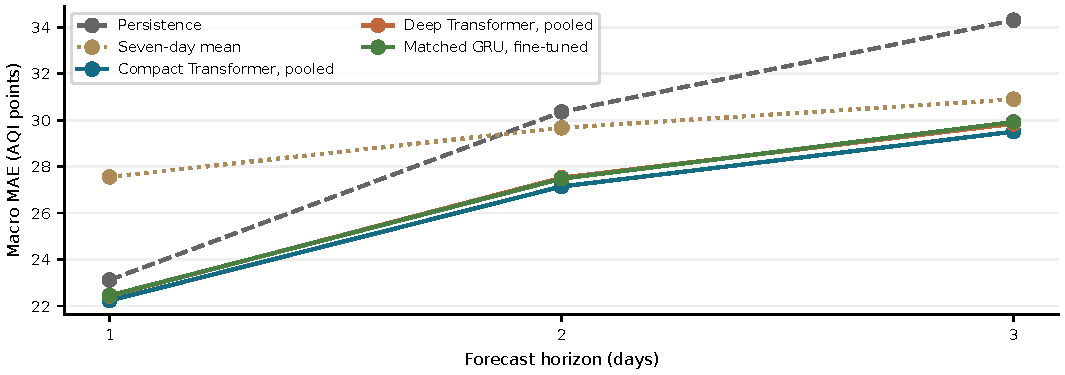
\includegraphics[width=.88\textwidth]{horizon_comparison.pdf}
\caption{2025 macro MAE at $B=90$. Pooled models are independent of the target fitting budget. Increasing horizon strengthens the advantage of pooled prediction over persistence. Lines join separately evaluated direct horizons.}
\label{fig:horizons}
\end{figure*}

\subsection{Fine-tuning helps local models but can hurt pooling}
Fine-tuning reduces matching local MAE in 40/45 compact cells and 48/54 expanded cells. It reduces local RMSE in 45/45 and 51/54, respectively. Yet the strict original condition holds in 0/99 cells. The failure arises because the full requirement includes a useful local model and improvement over persistence, not merely a favorable fine-tuned-versus-local difference.

The distinction is substantial for larger networks. At $B=90$ and one day, deep GRU fine-tuning reduces local MAE from 31.93 to 28.80, but the pooled GRU without target fitting scores 22.45. Deep LSTM fine-tuning reduces local MAE from 32.83 to 26.96, while its pooled model scores 23.21. These results are consistent with harmful adaptation under a small, recent target sample. They do not prove a particular overfitting mechanism without additional controls.

The matched GRU changes much less. At $B=90$, fine-tuning gives MAE 22.454 versus pooled 22.483 at one day, a paired difference of $-0.029$ with 95\% interval $[-0.133,0.031]$. Its difference from persistence is $-0.670$ with interval $[-1.409,0.031]$; four cities improve and two worsen. At two and three days, its fine-tuned MAE is 27.48 and 29.92. Small mean improvements over pooling should not be presented as a uniformly reliable next-day adaptation gain.

\subsection{Matched meta-learning comparisons}
Full MAML, FOMAML and Reptile with native SGD have lower macro MAE than ordinary matched fine-tuning in 0/27 prespecified main-test cells. None of the corresponding intervals lies wholly below zero. Fig.~\ref{fig:meta} shows the differences by budget and horizon. At $B=90$, MAML minus ordinary transfer is $1.044$ AQI points at one day (95\% interval $[0.477,1.307]$), $0.360$ at two days ($[-0.217,0.638]$), and $0.240$ at three days ($[-0.384,0.742]$). Three-day similarity at this budget is not evidence that MAML improves the control.

Second-order MAML has lower macro MAE than FOMAML in 3/9 cells; only one unadjusted interval lies wholly below zero. MAML outperforms Reptile in 6/9, especially at longer horizons, but superiority to Reptile does not establish an advantage over ordinary transfer. Changing final meta adaptation to the donor-selected Adam schedules gives lower MAE than corresponding SGD in 0/27 cells. Since optimizer and schedule change together, this is not an isolated optimizer effect.

\begin{figure*}[t]
\centering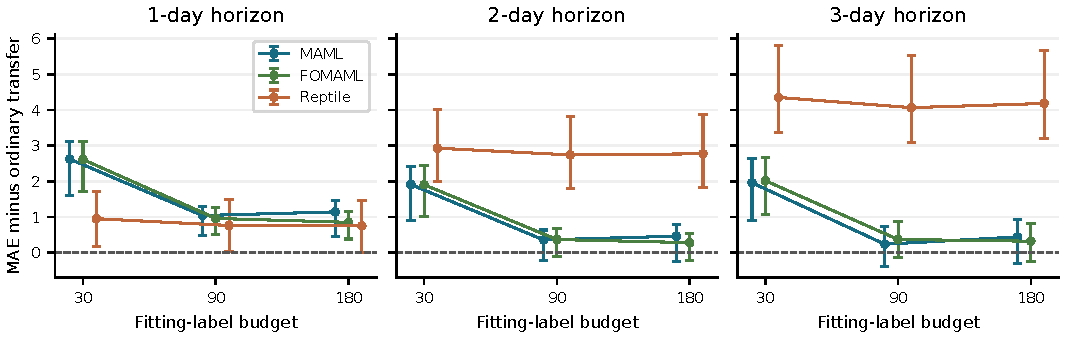
\includegraphics[width=.97\textwidth]{meta_comparison.pdf}
\caption{Meta-learning minus matched ordinary transfer in 2025. Positive differences favor ordinary transfer. Error bars are paired 95\% calendar-block intervals conditional on the selected cities, unadjusted for multiple comparisons. All 27 point estimates are positive.}
\label{fig:meta}
\end{figure*}

The six-donor ablation has lower MAE than the corresponding full-pool arm in 9/27 cells, with three favorable intervals. Those three occur for MAML at $B=30$. Ordinary pooled and fine-tuned six-donor models do not produce a consistent gain. Task count, unique data and donor composition change jointly, so these results do not show that fewer donors generally improve meta-learning or identify a transferable pollution mechanism.

\subsection{Capacity, time sensitivity and computation}
Larger models are not uniformly better. The expanded pooled GRU improves over its compact counterpart at one day, but the expanded pooled Transformer is worse than the compact Transformer at all three horizons. Deep local and fine-tuned models can be markedly worse. This comparison concerns a capacity-and-optimization package, not a randomized intervention on parameter count.

The secondary 2024 evaluation uses the same fitted weights. For example, at $B=30$ and one day, matched fine-tuning minus persistence changes from $-0.838$ in 2024 to $-0.488$ in 2025; MAML minus matched fine-tuning changes from $0.911$ to $2.626$. Both retain their directions but vary in magnitude. Neither year was used to tune settings. Between-year differences may combine environmental variation, missing-window selection and model aging; the experiment does not identify their separate causes.

The compact CPU run retains 1,876,662 forecast records and 1,644 fitting records; the expanded Apple GPU run retains 2,692,602 and 3,003. These records include repeated methods, seeds, budgets and horizons. Expanded summed fitting elapsed time is approximately 9,543 s, including donor validation, checkpoint work and resumed fitting time. The final invocation wall time is approximately 9,287 s.

\section{Post-Hoc Adaptation and Objective Controls}
\label{sec:followup}
We froze the control grid after seeing the primary results. We reused the six cities, their original fitting labels, and the exact 2024 and 2025 forecast windows. We report every schedule and replay the archived forecasts to verify the starting checkpoints. For selected contrasts, we use 4,000 resamples of 14- and 28-day calendar blocks with shared block draws across cities. The 95\% intervals condition on these six cities and describe temporal uncertainty in the inspected years.

\subsection{Support fit and future error}
We record the original target-update trajectory for the deeper and matched GRUs across all cities, budgets and seeds. Additional controls reduce the learning rate tenfold, freeze all but the output head, or penalize squared parameter movement from the pretrained weights ($\lambda=0.01$ or $0.1$)~\cite{l2sp}. The controls use the original support batches and optimizer for each backbone. The 216 zero-step and original-endpoint replay checks agree with archived forecasts within $1.2\times10^{-5}$ AQI points.

The deep pooled GRU starts at 26.669 macro MAE in 2025, averaged across the budgets and horizons. After its original 100 Adam updates at 0.0003, MAE rises by 10.960 points in 2025 (14-day block interval $[8.813,12.991]$) and by 8.579 in 2024. The 2025 increases at 30, 90 and 180 labels are 21.381, 8.250 and 3.248; larger budgets also extend the support window. Mean residual MSE on the fitting labels falls by 0.0672 in scaled units. The support MSE falls and 2025 MAE rises together in 149/162 city--budget--seed--horizon cases. MAE also rises by 9.356 on the fixed donor refit panel, which measures retention of donor training performance.

For initial error $e=\widehat y_0-y$ and adaptation correction $d=\widehat y_1-\widehat y_0$, the change in squared error is $2ed+d^2$. In 2025 the mean cross term is $-132.0$ AQI$^2$, indicating that the correction has a favorable mean projection against the initial errors. Its mean squared size is $1,224.7$ AQI$^2$, which dominates and raises MSE by $1,092.7$ AQI$^2$. This shows that large changes are sufficient to account for the net squared-error increase even when their aggregate direction is favorable.

At the same 100 updates, the 2025 MAE rise shrinks to 0.606 with the lower learning rate, 1.853 with head-only adaptation, and 7.021 or 3.371 with the weaker or stronger weight anchor (Fig.~\ref{fig:adaptationdiagnostics}). Each control limits parameter movement. The matched GRU's original three SGD updates at 0.01 change 2025 MAE by only $+0.008$ (14-day block interval $[-0.089,0.114]$), while thirty updates raise it by 0.724. The interventions trace much of the deep-GRU loss to the size and freedom of the target update. The experiment leaves the environmental source of the support-to-query difference open.

\begin{figure}[t]
\centering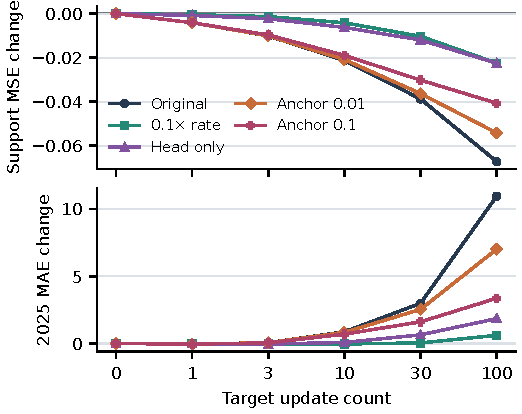
\includegraphics[width=\columnwidth]{adaptation_diagnostics.pdf}
\caption{Deep-GRU changes from the pooled checkpoint. The support panel shows scaled residual MSE and the 2025 panel shows AQI MAE. Both average across cities, budgets, horizons and seeds. Checkpoint positions are equally spaced on the axis.}
\label{fig:adaptationdiagnostics}
\end{figure}


\subsection{Learning-rate control across architectures}
We repeated the tenfold learning-rate reduction for the other four architectures at their released 100-update Adam schedule. Each pair shares a starting checkpoint, sampled training batches and evaluation windows. The only intervention is the rate ($3\times10^{-4}$ versus $3\times10^{-5}$). We examine every combination of six cities, three fitting budgets, three horizons and three seeds.

\begin{table}[t]
\caption{2025 macro MAE and its change after 100 target updates. Changes are relative to each row's pooled MAE and expressed in AQI points. Positive values mean higher error.}
\label{tab:architecture-rate}
\centering\small
% Generated from the verified CSV files in figure_data/.
\begin{tabular}{lrrr}\toprule
Architecture & Pooled MAE & Original $\Delta$ & $0.1\times$ rate $\Delta$ \\\midrule
Wider GRU & 26.67 & +10.96 & +0.61 \\
LSTM & 29.17 & +4.38 & +0.08 \\
MLP & 27.10 & +10.45 & +2.09 \\
TCN & 26.65 & +15.73 & +1.01 \\
Transformer & 26.60 & +13.12 & +1.38 \\
\bottomrule
\end{tabular}

\end{table}

The original updates lower target fitting MAE across all five architectures and raise 2025 MAE by 4.38--15.73 points. At one-tenth the rate, the increases fall to 0.08--2.09 points (Table~\ref{tab:architecture-rate}). For each added architecture, the original squared correction term $d^2$ dominates the favorable mean cross term $2ed$. Reducing the rate shrinks $d^2$ across all four. The four 2024 MAE penalties also fall, from 3.40--13.34 to $-0.04$--1.45 points. These interventions identify a source of error for the released schedules. A fresh evaluation is needed to assess the reduced rate on unseen dates.


\subsection{Matched target updates}
For the pooled, MAML, FOMAML and Reptile GRU checkpoints, we held target-label batches and SGD fixed and recorded predictions at zero, one, three, ten and thirty updates. The two learning rates were 0.01 and 0.03. The 270 replays of original pooled and adapted forecasts agree within $3\times10^{-5}$ AQI points.

\begin{table}[t]
\caption{2025 MAE in AQI points, averaged equally over cities, budgets, horizons and seeds. Each row uses the same target updates within that row. The middle rows are the original pooled and MAML schedules, applied to all four initializations.}
\label{tab:matchedupdates}
\centering\small
\begin{tabular}{lrrrr}\toprule
SGD & Pooled & MAML & FOMAML & Reptile\\\midrule
Zero updates & 26.677 & 28.267 & 27.406 & 29.054\\
$0.01\times3$ & 26.685 & 27.739 & 27.221 & 29.066\\
$0.03\times10$ & 27.498 & 27.819 & 27.764 & 29.299\\
$0.03\times30$ & 28.505 & 28.807 & 28.817 & 29.587\\\bottomrule
\end{tabular}
\end{table}

Pooled starts 1.590 MAE points ahead of MAML in 2025 (14-day block interval $[0.956,2.264]$) and retains the lowest aggregate MAE at every common setting. MAML improves on its own initialization at seven of the eight nonzero schedules. At the original MAML setting ($0.03\times10$), its MAE drops 0.448, while pooled MAE rises 0.821. The original gap with distinct schedules is 1.134 points. Giving both $0.03\times10$ makes the gap 0.321 (14-day block interval $[0.028,0.623]$), while giving both $0.01\times3$ makes it 1.054. FOMAML improves on its own initialization at five of eight schedules. Reptile changes little at its shortest setting and deteriorates at longer schedules.

The ranking varies by year. In 2024, MAML errors are 0.159 and 0.145 points lower than pooled errors at the shared $0.01\times30$ and $0.03\times10$ settings. The interval for the latter difference includes zero ($[-0.408,0.115]$). At $0.03\times30$ in 2025, pooled support MSE falls and query MAE rises in 128/162 paired city--budget--seed--horizon cases.

\subsection{What produced MAML's starting deficit?}
We train two copies of the same GRU from identical weights using the archived donor task stream, with three seeds and 1,350 outer updates per seed. The query examples are identical across copies. One objective evaluates query loss immediately. The other evaluates it after five updates on the corresponding local support examples, reproducing full MAML. All 16,200 archived task records are replayed. Reproduced MAML forecasts agree with the release within $2.6\times10^{-5}$ AQI points.

\begin{table}[t]
\caption{2025 macro MAE in AQI points before and after five shared local SGD steps ($\eta=0.03$). The paired-task rows isolate the source objective. The broader-dates row changes the query-date sampling under immediate loss.}
\label{tab:objective}
\centering\small
% Generated from the verified CSV files in figure_data/.
\begin{tabular}{lrr}\toprule
Source training & Zero steps & Five steps \\\midrule
Released pooled GRU & 26.68 & 27.14 \\
Immediate loss, paired tasks & 26.94 & 27.45 \\
Post-update loss (MAML) & 28.27 & 27.56 \\
Immediate loss, broader dates & 26.82 & 27.47 \\
\bottomrule
\end{tabular}

\end{table}

The immediate objective lowers zero-step error by 1.326 points in 2025 (14-day block interval $[0.722,1.980]$). This accounts for about 83\% of the 1.590-point difference between released MAML and pooled GRU. After five shared updates, the paired gap shrinks to 0.111 points ($[-0.233,0.465]$). The analogous five-step gap in 2024 is $-0.159$ ($[-0.425,0.086]$). The broad-date control lowers 2025 zero-step MAE by a further 0.122 points ($[-0.074,0.302]$). These paired comparisons explain much of the starting gap in this GRU and task stream. The post-update differences remain imprecise.


\subsection{Donor composition under equal source volume}
The original six-donor ablation reduced both donor count and available data. We add three paired chains of nested panels with 6, 12 or 23 cities. Each panel contains 3,312 city--label dates (9,936 horizon pairs) and identical year totals. Within each chain, counts share a training seed. Pooled training uses 1,200 updates per panel. MAML uses 300 outer updates with 90-label support, a 14-label query and the original calendar purge. The original MAML refit used 1,350 outer updates with multiple support budgets. We score each panel before target adaptation and after the same two SGD schedules.

In 2025, increasing from 6 to 23 donors lowers pooled MAE by 0.473--0.907 points across schedules and raises MAML MAE by 0.186--0.329. These directions hold in all three chains for the 6-to-23 comparison. The 12-donor panel has the lowest MAML mean across chains at each schedule. Narrower panels include more dates per donor. City identities, per-city temporal density, unique lag context and episode spans vary with panel width. The result describes sensitivity to these donor panels and shorter MAML training. A general minimum donor count remains unresolved.


\section{Reproducibility and Limitations}
Code and reproducibility materials are available at \url{https://github.com/arjunsrikanthh/afml-course-project}. Release \texttt{study-v1.0.0} includes four executed notebooks, weights, forecasts and data manifests. Release \texttt{extension-v1.0.0} provides the frozen cross-architecture and objective protocols, run scripts and numeric evidence. The archived source data have SHA-256 prefix \texttt{014fa6ab88854a96} and the frozen expanded engine has prefix \texttt{7e8c51383d43715d}. Figures and new tables can be regenerated from the bundled results.

An independent artifact audit passes nine checks for the compact study and twelve for the expanded study, with zero critical failures. Checks cover source checksums, whole-city exclusions, legal features and truth, nested budgets, fitting chronology, donor-only candidate rankings, explicit target label sets, recorded derivative evidence and recomputed city/seed and macro metrics. The expanded audit does not import or rerun the model engine. Its scope is artifact consistency, chronology and metric reconstruction; it does not prove every declared hardware update, independently reparse all workbook cells with a second parser, or certify bootstrap interpretation. This distinction bounds what ``verified'' means.

The initial follow-up audit validates receipt hashes, query and support rows, and recomputed metrics across 540 adaptation blocks and 216 initialization blocks. All 31 original artifact hashes agree with their initial snapshot. In the extension, the architecture audit covers 432 trajectory blocks and 5,767,200 forecasts. The objective audit recomputes results from 1,631,880 stored forecasts at zero and five local updates.

Several limits constrain external validity. Six targets cannot establish nationwide generalization. Annual availability screening selects well-reported stations, and common complete windows leave only 133 and 135 main-test dates in Ahmedabad and Guwahati. Scarcity is simulated by withholding fitting labels while retaining recent context, so naturally sparse monitors may behave differently. The latest-$B$ design confounds sample size with recency and season. One monitor per city is not a city average. Current metadata and coordinates cannot resolve all historical station changes.

Only seven AQI lags and calendar features are used. We do not test longer histories, verified weather forecasts, causal transport, spatial graphs or publication-time revisions. Frozen 2023 fitting is useful for a controlled comparison but differs from routine rolling refits. Hyperparameter searches can overfit donor validation, and finite optimization is not proof of optimal training. Temporal bootstrap intervals hold cities fixed and do not adjust for multiple testing. Negative findings therefore concern these implementations, tasks and schedules, rather than rule out meta-learning for air quality.

The diagnostic controls explain how the fitted models changed on the observed examples. Fresh target cities and later issue dates would test whether the same patterns recur. Operational evaluation would also require publication-time evidence and rolling refits.

\section{Conclusion}
Pooled cross-city forecasts show their clearest gains over persistence at two and three days. The original joint MAE/RMSE criterion holds in 0/99 cells. Across five architectures, the original fine-tuning schedule fits the local training sample more closely and worsens 2025 forecasts. A tenfold smaller learning rate reduces that penalty in every architecture. On the archived MAML task stream, training for error after local updates explains most of the weaker starting forecasts. The paired difference is small after five shared updates and varies by year.

\balance
\section*{Author Contributions}
Ankit Umadi conducted background research and collected and prepared the data. Arjun Srikanth implemented and trained the models and ran the benchmarks. Jayanth K carried out the follow-up experiments, verification and reporting.

\begin{thebibliography}{11}
\bibitem{cpcb_report} Central Pollution Control Board, \emph{National Air Quality Index}, Control of Urban Pollution Series CUPS/82/2014-15, 2014. [Online]. Available: \url{https://airquality.cpcb.gov.in/ccr_docs/FINAL-REPORT_AQI_.pdf}
\bibitem{cpcb_data} Central Pollution Control Board, ``AQI repository,'' Central Control Room for Air Quality Management. Source snapshot: Nov. 14, 2026. [Online]. Available: \url{https://airquality.cpcb.gov.in/ccr/#/repository/aqi}
\bibitem{regiontrans} L. Wang, X. Geng, X. Ma, F. Liu, and Q. Yang, ``Cross-city transfer learning for deep spatio-temporal prediction,'' in \emph{Proc. IJCAI}, 2019, pp. 1893--1899, doi: 10.24963/ijcai.2019/262.
\bibitem{poelzl} M. Poelzl, R. Kern, S. Kecorius, and M. Lovri\'{c}, ``Exploration of transfer learning techniques for the prediction of PM$_{10}$,'' \emph{Scientific Reports}, vol. 15, art. 2919, 2025, doi: 10.1038/s41598-025-86550-6.
\bibitem{cho} K. Cho et al., ``Learning phrase representations using RNN encoder--decoder for statistical machine translation,'' in \emph{Proc. EMNLP}, 2014, pp. 1724--1734, doi: 10.3115/v1/D14-1179.
\bibitem{lstm} S. Hochreiter and J. Schmidhuber, ``Long short-term memory,'' \emph{Neural Computation}, vol. 9, no. 8, pp. 1735--1780, 1997, doi: 10.1162/neco.1997.9.8.1735.
\bibitem{tcn} S. Bai, J. Z. Kolter, and V. Koltun, ``An empirical evaluation of generic convolutional and recurrent networks for sequence modeling,'' arXiv:1803.01271, 2018.
\bibitem{transformer} A. Vaswani et al., ``Attention is all you need,'' in \emph{Advances in Neural Information Processing Systems}, vol. 30, 2017.
\bibitem{maml} C. Finn, P. Abbeel, and S. Levine, ``Model-agnostic meta-learning for fast adaptation of deep networks,'' in \emph{Proc. ICML}, PMLR, vol. 70, 2017, pp. 1126--1135.
\bibitem{reptile} A. Nichol, J. Achiam, and J. Schulman, ``On first-order meta-learning algorithms,'' arXiv:1803.02999, 2018.
\bibitem{l2sp} X. Li, Y. Grandvalet, and F. Davoine, ``Explicit inductive bias for transfer learning with convolutional networks,'' in \emph{Proc. ICML}, PMLR, vol. 80, 2018, pp. 2825--2834.
\end{thebibliography}
\end{document}
